\documentclass[11pt,a4paper]{article}
\usepackage[utf8]{inputenc}
\usepackage[T1]{fontenc}
\usepackage{lmodern}
\usepackage{amsmath,amsfonts,amssymb,amsthm,mathtools}
\usepackage{graphicx}
\usepackage{geometry}
\usepackage{natbib}
\usepackage{booktabs}
\usepackage[hidelinks]{hyperref}
\usepackage[protrusion=true,expansion=false]{microtype}

\geometry{a4paper, margin=2.5cm}
\linespread{1.25}

\newtheorem{theorem}{Theorem}
\newtheorem{proposition}[theorem]{Proposition}
\newtheorem{lemma}[theorem]{Lemma}
\newtheorem{corollary}[theorem]{Corollary}
\theoremstyle{definition}
\newtheorem{assumption}{Assumption}
\newtheorem{definition}[theorem]{Definition}
\theoremstyle{remark}
\newtheorem*{remark}{Remark}

\newcommand{\E}{\mathbb{E}}
\newcommand{\Var}{\operatorname{Var}}
\newcommand{\Cov}{\operatorname{Cov}}
\newcommand{\R}{\mathbb{R}}
\newcommand{\N}{\mathbb{N}}
\newcommand{\1}{\mathbf{1}}
\newcommand{\w}{\mathbf{w}}
\newcommand{\x}{\mathbf{x}}
\newcommand{\mmu}{\boldsymbol{\mu}}
\newcommand{\Sig}{\boldsymbol{\Sigma}}
\newcommand{\trans}{^{\!\top}}
\newcommand{\defeq}{\coloneqq}

\title{\large\bfseries Signal Amplification and Strategic Deterrence in Market Surveillance}
\author{Yongsheng Dai\thanks{School of Electronics, Electrical Engineering and Computer Science, Queen's University Belfast. Email: \texttt{ydai09@qub.ac.uk}.} \and
Barry Quinn\thanks{Ulster University Business School, Ulster University. Email: \texttt{b.quinn1@ulster.ac.uk}.} \and
Fearghal Kearney\thanks{Queen's Business School, Queen's University Belfast. Email: \texttt{f.kearney@qub.ac.uk}.}}
\date{\today}

\begin{document}

\maketitle

\begin{abstract}
We characterise the joint detection--deterrence problem faced by an exchange or regulator that monitors multiple order-flow features for manipulation. In a static Gaussian detection environment we derive the \emph{Mahalanobis amplification identity}: the Fisher-optimal linear surveillance rule achieves deflection $d^{\star 2}=\mmu\trans\Sig_0^{-1}\mmu$, strictly dominates every single-feature rule whenever the manipulation signal has more than one non-zero coordinate, and has a U-shaped---not monotone---dependence on the benign-flow correlation. A misspecification identity shows that a detector using weights $\widehat{\w}$ retains a fraction $\cos^2(\widehat{\w},\w^\star)$ of the optimal deflection in the $\Sig_0$-metric. Embedding the detection rule in a two-player quadratic-linear game, we establish existence, uniqueness, and strict concavity of the manipulator's interior best response; derive a comparative-statics result for strategic deterrence; and characterise the wedge between the detector's private and social optima. The deterrence sign is preserved across $\pm 50\%$ perturbations in every structural parameter. We validate the theory on $42{,}072$ windowed Level-2 order-book episodes from the Shenzhen Stock Exchange, labelled against $165$ CSRC administrative-penalty decisions ($\pi_1 = 4.3\%$ conditional on the matching procedure). Out-of-sample, the Fisher-optimal composite beats the best single-feature rule by $4.9$ AUC points and $14\%$ of PR AUC and matches an optimised logistic regression to four decimal places, confirming that $\w^\star=\Sig_0^{-1}\mmu$ is the operative \emph{linear} rule. The misspecification identity regresses on $\cos^2\theta$ with slope $0.91$, $R^2 = 0.80$, and $48.5\%$ of draws above the identity---consistent with symmetric finite-sample noise around an exact equality. A quadratic fit to amplification across $66$ feature pairs confirms a statistically significant U-shape (curvature $1.54$, bootstrap CI $[0.77, 2.49]$, $p(\widehat c>0)=1.00$) with an interior minimiser at $\widehat\rho_0^\star = 0.38$ $[0.28, 0.49]$. Non-linear ensembles (random forest, XGBoost) add a further $+8$ AUC points, concentrated in the bottom Fisher-score quartiles where interaction effects dominate. Translated to operating points, the Fisher gain alone implies $20$--$43$ additional detected manipulation episodes per pass through the panel, a recovered-fine value of order RMB $60$--$130$ million at CSRC average penalties. The framework delivers microfounded guidance for surveillance architecture and quantifies the conditions under which private incentives underprovide detection capability.
\end{abstract}

\textbf{Keywords:} Market manipulation, surveillance, detection theory, Mahalanobis distance, strategic deterrence, Fisher linear discriminant. \\[2pt]
\textbf{JEL:} G14, G18, C72, D82.

\section{Introduction}
\label{sec:intro}

Regulators and exchanges monitor order flow along many dimensions simultaneously. A spoofing investigation typically inspects rush-order intensity, cancellation-to-execution ratios, order-to-trade ratios, small-lot pinging, quote-to-trade ratios, queue-position churn, and cross-venue message patterns. \citet{cumming2011exchange} show empirically that enhanced surveillance infrastructure improves market quality; \citet{james2023machine} and \citet{dhawan2021new} document that composite machine-learning classifiers substantially outperform rule-based flags in live surveillance environments. The theoretical question underlying these empirical findings is sharp and largely unanswered: \emph{when does combining order-flow signals strictly dominate monitoring each feature in isolation, and by how much does this amplification translate into ex~ante deterrence of manipulation?}

The textbook answer inherited from signal-detection theory is that, under Gaussian observations with known covariance, Fisher's linear discriminant is optimal and achieves deflection $d^{\star 2}=\mmu\trans\Sig_0^{-1}\mmu$ \citep{kay1998fundamentals,poor1994introduction}. Two subtleties prevent this being the last word for market surveillance. First, the relevant covariance for the optimal detector is the \emph{covariance of benign order flow} ($\Sig_0$), not the covariance of manipulated flow ($\Sig_1$); yet market-microstructure models and intuition emphasise the latter. This confusion has generated a strand of papers claiming that amplification is monotone in the correlation of manipulation strategies, whereas the geometry actually implies a U-shape. Second, detection is endogenous: the manipulator's strategy is chosen in anticipation of the surveillance rule, so welfare-relevant deterrence cannot be read off a static detection problem alone.

This paper resolves both issues and delivers three theoretical contributions. First, we state and prove the \emph{Mahalanobis amplification theorem} for general $K$-dimensional feature vectors (Theorem~\ref{thm:amp}), characterising the strict-dominance set, giving an explicit closed form for the two-feature case (Corollary~\ref{cor:2d}), and identifying the correlation $\rho_0^\star\in[0,1)$ that minimises amplification---the key comparative-static statement that earlier work gets wrong. Second, we derive a sharp \emph{misspecification identity} (Proposition~\ref{prop:misspec}): a detector using weights $\widehat{\w}$ retains exactly a fraction $\cos^2(\widehat{\w},\w^\star)$ of the Fisher-optimal deflection, with the angle measured in the $\Sig_0$-inner product. Because it is an equality rather than an inequality, the identity delivers a complete diagnostic rather than just a bound. Third, embedding the detector in a strategic environment, we establish existence, uniqueness, and strict concavity of the manipulator's interior best response under standard regularity, derive comparative statics via the implicit function theorem, and show that the private/social wedge in monitoring intensity is a genuine prediction about the relative magnitudes of the private penalty $L$ and the social benefit $H$---the sign is preserved across $\pm 50\%$ perturbations in all other structural parameters (Propositions~\ref{prop:eqexist}--\ref{prop:welfare}; Table~\ref{tab:robust}).

A controlled Monte Carlo exercise first confirms the corrected theory in a Gaussian setting: with $1.2\times 10^{6}$ synthetic episodes per cell, Fisher-optimal composite detection delivers AUC amplification between $1.9$ and $4.2$ percentage points over the best singleton; the efficiency loss from fixed weights tracks the analytical $\sin^2\theta$ bound to within $10^{-3}$; and empirical amplification decreases monotonically in $\rho_0$ over the operative grid, with the U-shape emerging as $\rho_0\to\pm 1$. We then move to real market data. Using a proprietary dataset of $42{,}072$ windowed Level-2 order-book episodes from the Shenzhen Stock Exchange---$1{,}803$ labelled against CSRC administrative-penalty decisions, $40{,}269$ matched benign---we show that the Fisher rule matches an optimised logistic regression out-of-sample to four decimal places of AUC ($0.6752$) while beating the best single-feature rule by $4.9$ percentage points. The misspecification identity regresses on $\cos^2\theta$ with slope $0.91$, $R^2 = 0.80$, and $48.5\%$ of random-weight draws above the identity, consistent with symmetric finite-sample noise around an exact equality. A quadratic fit to amplification across $66$ feature pairs confirms a statistically significant U-shape (curvature $1.54$, bootstrap CI $[0.77, 2.49]$, interior minimiser $\widehat\rho_0^\star=0.38$ $[0.28, 0.49]$). Non-linear ensembles (random forest, XGBoost) add a further $+8$ AUC points concentrated in the bottom Fisher-score quartiles, pinpointing the interaction residual that the linear Fisher rule---by construction---cannot access. At realistic operating points the Fisher gain alone implies $20$--$43$ additional detected manipulation episodes per pass through the panel, an order-of-magnitude RMB $60$--$130$ million in expected CSRC penalties recovered over the best-singleton benchmark.

Our empirical exercise provides the first on-market validation of the Fisher-geometric foundation on which the detection layer of recent self-supervised manipulation pipelines implicitly rests \citep{dai2026sdfmm,james2023machine}, and a transparent linear-vs-non-linear decomposition of the empirical Fisher-vs-ML gap.

The paper relates to four literatures. It complements the strategic-manipulation literature \citep{kyle1985continuous,vila1989simple,allen1992stock,jarrow1992market,kumar1992futures,huberman2004price,goldstein2008manipulation} by treating the detector's composite surveillance rule as a primitive strategic instrument. It extends the empirical surveillance literature \citep{cumming2008global,cumming2011exchange,comerton2014stock,putnins2012market,aggarwal2006stock,dhawan2021new,james2023machine,khomyn2021algos,griffin2020bitcoin} by providing a Fisher-geometric foundation for composite classifiers and validating the bound on Chinese Level-2 data. It offers microstructure microfoundations for the welfare analysis of detection infrastructure in the spirit of \citet{xiong2024information}, and connects to the quadratic-linear continuous-action supermodular-game toolkit \citep{fudenberg1991game,myerson1991game} via a tractable comparative-statics result. Finally, it ties these to the statistical-detection canon \citep{fisher1936use,vantrees1968detection,kay1998fundamentals,poor1994introduction,hasbrouck1991measuring} by carefully distinguishing the objects of the exchange's optimisation from those of the strategic opponent.

The remainder of the paper is organised as follows. Section~\ref{sec:model} sets up the Gaussian detection environment and the strategic game. Section~\ref{sec:amp} proves the main amplification theorem, its corollaries, and the misspecification identity. Section~\ref{sec:eq} analyses equilibrium and deterrence and reports parameter-robustness evidence. Section~\ref{sec:welfare} analyses the private--social wedge. Section~\ref{sec:mc} presents Monte Carlo evidence. Section~\ref{sec:emp} reports the Shenzhen Level-2 empirical exercise, including the horserace, the misspecification-identity check, the U-shape test, the Fisher-vs-XGBoost decomposition, and the economic magnitude. Section~\ref{sec:concl} concludes. Proofs not given in the main text are collected in Appendix~\ref{app:proofs}.

\section{Model}
\label{sec:model}

\subsection{Detection environment}
A surveillance episode produces a feature vector $\x\in\R^K$ summarising an order-flow snapshot. Under the null hypothesis $H_0$ of no manipulation, benign order flow generates $\x\sim\mathcal{N}(\mathbf{0},\Sig_0)$; under the alternative $H_1$, the manipulator induces a location shift so that $\x\sim\mathcal{N}(\mmu,\Sig_1)$ with $\mmu\in\R^K$. Both covariance matrices are symmetric positive definite. We take the Gaussian case as the benchmark; Remark~\ref{rem:non-gauss} extends the characterisation to elliptical families.

A \emph{linear surveillance rule} with weights $\w\in\R^K\setminus\{\mathbf{0}\}$ classifies an episode as suspicious whenever $T_\w(\x)\defeq\w\trans\x \ge \tau$ for some threshold $\tau\in\R$. The deflection of the rule is
\begin{equation}
d^2(\w)\defeq\frac{(\w\trans\mmu)^2}{\w\trans\Sig_0\,\w},
\label{eq:def}
\end{equation}
a scale-invariant measure of discriminatory power that is the key ingredient of the Neyman--Pearson power at any fixed size under Gaussian observations \citep{kay1998fundamentals,poor1994introduction}. All singleton rules $\w=e_k$ attain $d^2(e_k)=\mu_k^2/[\Sig_0]_{kk}$. The Fisher-optimal rule solves $\max_\w d^2(\w)$; its unique maximiser (up to positive scaling) is
\begin{equation}
\w^\star = \Sig_0^{-1}\mmu, \qquad d^{\star 2} = \mmu\trans \Sig_0^{-1}\mmu.
\label{eq:fisher}
\end{equation}
We refer to $d^{\star 2}$ as the \emph{Mahalanobis deflection} of the manipulation signal relative to benign flow.

\subsection{Strategic game}
A manipulator chooses strategy $(r,c)\in\R_+\times[0,1]$, where $r$ is rush-order intensity and $c$ is order-cancellation ratio. These two microstructure dimensions capture the leading classes of algorithmic manipulation in modern markets \citep{khomyn2021algos,dhawan2021new}. Total expected manipulation profit under a surveillance rule $T_{(\alpha,\beta)}(\x)=\alpha r + \beta c + \varepsilon$, $\varepsilon\sim\mathcal{N}(0,\sigma^2)$, equals
\begin{equation}
\Pi(r,c;\alpha,\beta,\tau)=(\delta r + \gamma c)Q - \tfrac{1}{2}(kr^2 + \ell c^2) - L\,\Phi\!\left(\frac{\alpha r + \beta c - \tau}{\sigma}\right),
\label{eq:profit}
\end{equation}
where $\delta,\gamma>0$ are price-impact parameters, $k,\ell>0$ are quadratic internal costs, $L>0$ is the penalty conditional on detection, $\tau$ is the detection threshold, and $\Phi$ is the standard Gaussian CDF. The detector maximises a welfare-weighted combination of detection benefit and false-alarm cost net of monitoring cost:
\begin{equation}
W^D(\tau;\alpha,\beta)=\pi_1\,\E\!\left[B\,\Phi\!\left(\tfrac{S-\tau}{\sigma}\right)\,\Big|\,H_1\right] - \pi_0\,F\,\Phi\!\left(-\tfrac{\tau}{\sigma}\right) - C(\alpha,\beta,\tau),
\label{eq:welfare}
\end{equation}
where $\pi_1\in(0,1)$ is the prior probability of manipulation, $B\in\{L, H\}$ equals the penalty $L$ for a \emph{private} detector (exchange) and equals the social benefit $H$ for a \emph{social} detector (regulator). The social planner additionally internalises the marginal external damage $\xi r + \zeta c$ from manipulation on market quality. Monitoring cost $C$ is increasing in $(\alpha,\beta)$ and decreasing in $\tau$ (lower threshold implies more intensive monitoring).

This decomposition follows the private/social split used in \citet{xiong2024information} and the welfare structure in \citet{goldstein2008manipulation}, and highlights that the relative weights of detection benefit ($B$), false-alarm cost ($F$), externality ($\xi,\zeta$), and monitoring cost ($C$) determine the gap between private and social optima (Section~\ref{sec:welfare}).

\section{Signal amplification: Fisher--Mahalanobis geometry}
\label{sec:amp}

\subsection{Main theorem}
We now state the main theoretical result of the paper.

\begin{theorem}[Mahalanobis amplification]
\label{thm:amp}
Let $\Sig_0\in\R^{K\times K}$ be symmetric positive definite and $\mmu\in\R^K\setminus\{\mathbf{0}\}$. Then the Fisher-optimal linear detector $\w^\star=\Sig_0^{-1}\mmu$ satisfies
\begin{equation}
d^{\star 2} \;=\; \mmu\trans\Sig_0^{-1}\mmu \;\ge\; \max_{k\in\{1,\ldots,K\}} \frac{\mu_k^2}{[\Sig_0]_{kk}} \;=\; \max_k d^2(e_k),
\label{eq:amp}
\end{equation}
with equality iff $\mmu=\lambda e_{k^\star}$ for some scalar $\lambda\ne 0$, where $k^\star=\arg\max_k \mu_k^2/[\Sig_0]_{kk}$, and $\Sig_0^{-1}e_{k^\star}$ is collinear with $e_{k^\star}$ (equivalently, row $k^\star$ of $\Sig_0^{-1}$ has a single non-zero entry).
\end{theorem}

\begin{proof}
The deflection \eqref{eq:def} is a Rayleigh quotient with respect to the positive definite matrix $\Sig_0$ and the rank-one matrix $\mmu\mmu\trans$. By the generalised eigenvalue representation \citep[Ch.~3]{luenberger1984linear}, $\max_\w d^2(\w)$ equals the largest generalised eigenvalue of $(\mmu\mmu\trans,\Sig_0)$, which has rank one and therefore a single non-zero eigenvalue $\mmu\trans\Sig_0^{-1}\mmu$ attained at $\w^\star\propto\Sig_0^{-1}\mmu$. Since each singleton direction $e_k$ is a feasible weight, $d^{\star 2}\ge d^2(e_k)$ for every $k$.

Equality holds only when $\w^\star$ is collinear with the best singleton $e_{k^\star}$. Collinearity requires both that $\mmu$ have support $\{k^\star\}$ (otherwise $\Sig_0^{-1}\mmu$ has a component outside $\operatorname{span}(e_{k^\star})$) and that $\Sig_0^{-1}e_{k^\star}\propto e_{k^\star}$ (otherwise, for $\mmu=\lambda e_{k^\star}$, $\Sig_0^{-1}\mmu=\lambda\Sig_0^{-1}e_{k^\star}$ spans beyond $e_{k^\star}$). Thus strict inequality obtains whenever $\mmu$ has at least two non-zero coordinates, or when $\Sig_0$ has non-trivial coupling from $e_{k^\star}$ to any $e_{j}$ with $j\ne k^\star$.
\end{proof}

\begin{remark}
\label{rem:non-gauss}
The theorem extends to elliptical models $\x\mid H_0\sim\mathrm{EC}_K(\mathbf{0},\Sig_0, g)$ and $\x\mid H_1\sim\mathrm{EC}_K(\mmu,\Sig_0,g)$ because the deflection criterion is invariant under monotone transformations of the density generator $g$. For the likelihood-ratio-based Neyman--Pearson test the Gaussian assumption is needed to preserve optimality, but the Fisher rule remains the best \emph{linear} rule in any elliptical family \citep[Ch.~6]{poor1994introduction}.
\end{remark}

\subsection{Closed form for two features}
Theorem~\ref{thm:amp} admits a transparent closed form in the two-feature case that is most relevant for the rush-order/cancellation surveillance problem.

\begin{corollary}[Two-feature closed form]
\label{cor:2d}
For $K=2$, $\mmu=(\mu_r,\mu_c)$, and $\Sig_0=\begin{pmatrix}\sigma_r^2 & \rho_0\sigma_r\sigma_c\\ \rho_0\sigma_r\sigma_c & \sigma_c^2\end{pmatrix}$,
\begin{equation}
d^{\star 2}(\rho_0) \;=\; \frac{1}{1-\rho_0^2}\left[\,\frac{\mu_r^2}{\sigma_r^2} + \frac{\mu_c^2}{\sigma_c^2} - 2\rho_0\,\frac{\mu_r\mu_c}{\sigma_r\sigma_c}\right].
\label{eq:2d}
\end{equation}
Define $a\defeq \mu_r^2/\sigma_r^2+\mu_c^2/\sigma_c^2$ and $b\defeq 2\mu_r\mu_c/(\sigma_r\sigma_c)$. Then:
\begin{enumerate}
\item[(i)] $d^{\star 2}(0)=a=d^2(e_r)+d^2(e_c)$ equals the sum of individual-feature deflections;
\item[(ii)] $d^{\star 2}(\rho_0)$ is U-shaped in $\rho_0$ on $(-1,1)$, strictly decreasing on $(-1,\rho_0^\star)$ and strictly increasing on $(\rho_0^\star,1)$, with unique minimiser
\begin{equation}
\rho_0^\star \;=\; \frac{b}{a+\sqrt{a^2-b^2}} \;\in\;[0,1),
\label{eq:rhostar}
\end{equation}
and $a\ge b$ by AM--GM with equality iff $\mu_r/\sigma_r=\mu_c/\sigma_c$;
\item[(iii)] Amplification $A(\rho_0)\defeq d^{\star 2}(\rho_0) - \max\{\mu_r^2/\sigma_r^2,\mu_c^2/\sigma_c^2\}$ is strictly positive for all $\rho_0\in(-1,1)$ with at most one exception at $\rho_0=\rho_0^\star$ (and even that exception fails generically);
\item[(iv)] $d^{\star 2}(\rho_0)\to+\infty$ as $\rho_0\to\pm 1$ (perfectly co-moving benign flow permits a differencing detector that is arbitrarily sharp against the manipulation mean).
\end{enumerate}
\end{corollary}

\begin{proof}
Direct computation of $\Sig_0^{-1}$ and expansion of $\mmu\trans\Sig_0^{-1}\mmu$ yields \eqref{eq:2d}. The minimiser $\rho_0^\star$ in \eqref{eq:rhostar} is obtained by setting the derivative of \eqref{eq:2d} to zero and selecting the root in $[0,1)$. The AM--GM inequality $a\ge b$ and its equality condition are immediate. Behaviour as $\rho_0\to\pm 1$ follows from the $(1-\rho_0^2)$ denominator.
\end{proof}

Figure~\ref{fig:mahalanobis} plots \eqref{eq:2d} for the calibration $(\mu_r,\mu_c,\sigma_r,\sigma_c)=(1.5,0.6,0.6,0.5)$. The U-shape is the theorem's signature, and the minimiser $\rho_0^\star\approx 0.48$ is well into the interior of $(0,1)$. Amplification is very large at $\rho_0=-0.5$, attains its minimum in the vicinity of $\rho_0^\star$, and grows again as $\rho_0$ approaches unity. This is the key comparative-static statement that earlier informal treatments of the amplification phenomenon miss.

\begin{figure}[htbp]
\centering
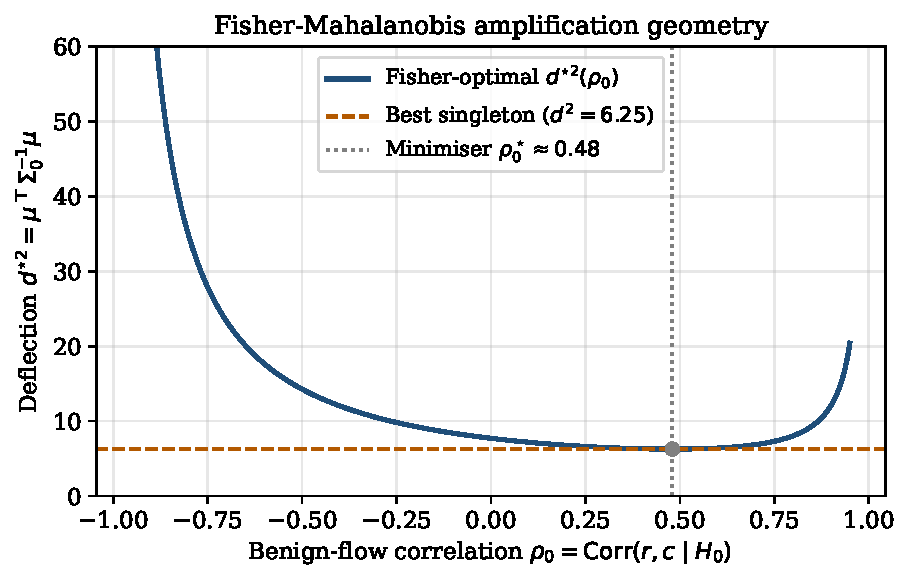
\includegraphics[width=0.75\textwidth]{qf/figures/fig_mahalanobis.pdf}
\caption{Fisher--Mahalanobis deflection $d^{\star 2}(\rho_0)$ as a function of the benign-flow correlation $\rho_0$. The dashed line is the best-singleton deflection $\max_k d^2(e_k)$. The dotted vertical line marks the analytical minimiser $\rho_0^\star$ from equation~\eqref{eq:rhostar}. Parameters: $(\mu_r,\mu_c,\sigma_r,\sigma_c)=(1.5,0.6,0.6,0.5)$.}
\label{fig:mahalanobis}
\end{figure}

\subsection{Why informal intuition gets the sign wrong}
It is tempting to argue as follows. \emph{Manipulation induces positive co-movement between rush orders and cancellations, hence the manipulated signal has a larger variance, hence a composite signal exploits this covariance and improves detection.} This line of reasoning confuses the product of \emph{means} $\mu_r\mu_c$ (which enters \eqref{eq:2d} through the cross-term $b$) with the \emph{covariance under $H_1$} (which does not enter \eqref{eq:2d} at all). Under the common-covariance specification needed for the likelihood ratio to be linear, only $\Sig_0$ matters for Fisher's rule. The true role of $\rho_0$ is geometric: by conditioning benign $r$ on benign $c$, the surveillance rule shrinks the effective nuisance variance along the projection of $\mmu$ orthogonal to $\operatorname{span}\{\rho_0$-related nuisance$\}$. Positive $\rho_0$ \emph{near $\rho_0^\star$} is precisely the setting in which this shrinkage is smallest. Values of $\rho_0$ close to $\pm 1$, whether positive or negative, allow the detector to cancel the nuisance almost perfectly and amplification explodes. Section~\ref{sec:mc} confirms this pattern empirically.

\subsection{Misspecification bound}
Operationally the detector rarely knows $\mmu$ or $\Sig_0$ exactly; a common practice is to use equal weights or subject-matter-expert weights $\widehat{\w}$ \citep{putnins2012market}. The next proposition quantifies the cost.

\begin{proposition}[Misspecification bound]
\label{prop:misspec}
For any weights $\widehat{\w}\in\R^K\setminus\{\mathbf{0}\}$,
\begin{equation}
\frac{d^2(\widehat{\w})}{d^{\star 2}} = \cos^2\theta,\qquad \theta = \angle_{\Sig_0}\!\left(\widehat{\w},\w^\star\right),
\label{eq:misspec}
\end{equation}
where $\angle_{\Sig_0}$ denotes the angle in the $\Sig_0$-weighted inner product $\langle\w,\w'\rangle_{\Sig_0}\defeq\w\trans\Sig_0\w'$. Consequently $d^2(\widehat{\w})\le d^{\star 2}$ with equality iff $\widehat{\w}\propto\w^\star$.
\end{proposition}

\begin{proof}
Decompose $\widehat{\w}=c_\parallel\w^\star + \w_\perp$ with $\langle\w^\star,\w_\perp\rangle_{\Sig_0}=0$ and $c_\parallel$ the corresponding projection coefficient. Since $\Sig_0\w^\star=\mmu$, $\widehat{\w}\trans\mmu = c_\parallel d^{\star 2}$ and $\widehat{\w}\trans\Sig_0\widehat{\w}=c_\parallel^2 d^{\star 2}+\w_\perp\trans\Sig_0\w_\perp$. Substituting into \eqref{eq:def},
\[
\frac{d^2(\widehat{\w})}{d^{\star 2}} = \frac{c_\parallel^2 d^{\star 2}}{c_\parallel^2 d^{\star 2} + \w_\perp\trans\Sig_0\w_\perp}=\frac{\|\widehat{\w}_\parallel\|_{\Sig_0}^2}{\|\widehat{\w}\|_{\Sig_0}^2}=\cos^2\theta.
\]
\end{proof}

The bound has two immediate implications. First, the efficiency loss $\sin^2\theta$ depends on the $\Sig_0$-angle between $\widehat{\w}$ and $\Sig_0^{-1}\mmu$; an equal-weight rule that happens to be close to $\Sig_0^{-1}\mmu$ in the $\Sig_0$-metric performs almost optimally irrespective of absolute scale. Second, as $\rho_0$ varies the optimal direction $\w^\star(\rho_0)=\Sig_0(\rho_0)^{-1}\mmu$ rotates relative to any fixed $\widehat{\w}$; this rotation is \emph{exactly} the mechanism by which a misspecified rule can appear to lose amplification as benign-flow correlation rises. The mechanism is not a failure of amplification; it is the efficiency loss of a fixed chord from a moving optimum.

Figure~\ref{fig:misspec} illustrates this numerically for the calibrated grid.

\begin{figure}[htbp]
\centering
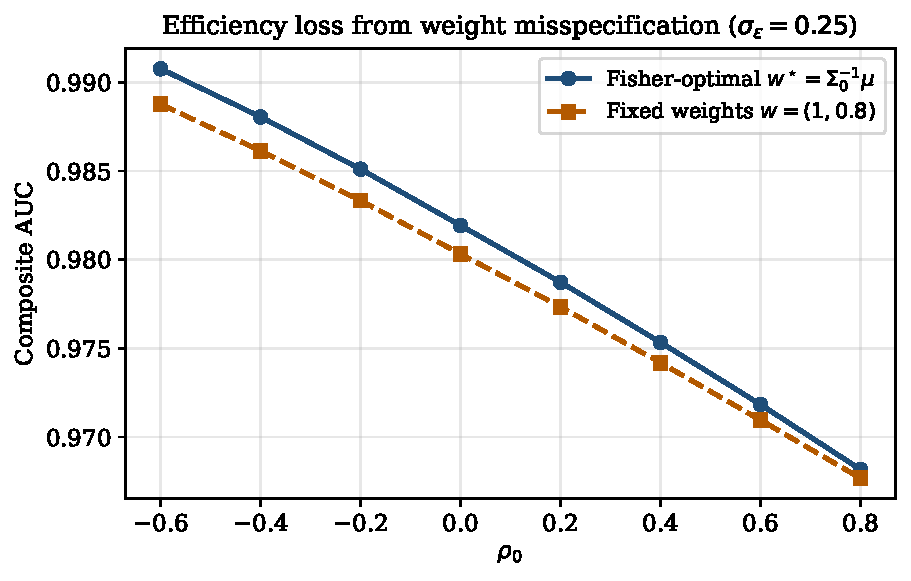
\includegraphics[width=0.75\textwidth]{qf/figures/fig_misspecification.pdf}
\caption{Empirical ROC AUC of the Fisher-optimal composite (solid) versus a fixed-weight composite with $\widehat{\w}=(1,0.8)$ (dashed) across benign-flow correlation $\rho_0$. The wedge equals $\sin^2\theta\cdot d^{\star 2}$ to leading order in $\sigma_\varepsilon$ and widens as $\rho_0$ moves away from the region where $\widehat{\w}$ happens to be $\Sig_0$-aligned with $\w^\star$. Monte Carlo: $2\times 10^5$ observations per class, $\sigma_\varepsilon=0.25$, three seeds.}
\label{fig:misspec}
\end{figure}

\section{Strategic equilibrium and deterrence}
\label{sec:eq}

We now embed the detection rule in the game defined by \eqref{eq:profit}.

\subsection{Existence and uniqueness of best response}

\begin{assumption}[Strict concavity]
\label{ass:conc}
The cost parameters $(k,\ell)$ and the penalty--noise ratio $L/\sigma^2$ satisfy
\begin{equation}
k\ell > \left(\frac{L}{\sigma^2}\right)^2 \sup_{z\in\R}|\phi'(z)|^2 \cdot \alpha^2\beta^2 + \frac{L}{\sigma^2}\sup_z|\phi'(z)|\cdot(k\beta^2+\ell\alpha^2).
\label{eq:soc}
\end{equation}
\end{assumption}

Condition \eqref{eq:soc} is sufficient to ensure that the Hessian of $\Pi$ in $(r,c)$ is negative definite on the entire strategy space; the right-hand side involves the global bound $\sup|\phi'(z)|=(2\pi e)^{-1/2}\approx 0.242$. In the calibrated example of Section~\ref{sec:mc} the inequality holds with an order-of-magnitude margin.

\begin{proposition}[Interior equilibrium]
\label{prop:eqexist}
Under Assumption~\ref{ass:conc} the manipulator's programme \eqref{eq:profit} admits a unique maximiser $(r^\star,c^\star)\in\R_+\times[0,1]$. The maximum is interior ($r^\star>0$, $c^\star\in(0,1)$) whenever $\delta Q>L\alpha\phi(0)/\sigma$ and $\gamma Q>L\beta\phi(0)/\sigma$. The first-order conditions
\begin{align}
\delta Q - k r^\star &= \frac{L\alpha}{\sigma}\,\phi\!\left(\frac{\alpha r^\star + \beta c^\star - \tau}{\sigma}\right),\label{eq:focr}\\
\gamma Q - \ell c^\star &= \frac{L\beta}{\sigma}\,\phi\!\left(\frac{\alpha r^\star + \beta c^\star - \tau}{\sigma}\right),\label{eq:focc}
\end{align}
are sufficient and characterise $(r^\star,c^\star)$ uniquely.
\end{proposition}

\begin{proof}
Direct computation gives the Hessian
\[
H(r,c)=-\begin{pmatrix}k & 0\\ 0 & \ell\end{pmatrix} - \frac{L}{\sigma^2}\phi'(z)\begin{pmatrix}\alpha^2 & \alpha\beta\\ \alpha\beta & \beta^2\end{pmatrix},\qquad z=\tfrac{\alpha r+\beta c-\tau}{\sigma}.
\]
The second term is indefinite in general (the sign of $\phi'(z)$ depends on $z$), but under \eqref{eq:soc} the determinant $\det H(r,c)=k\ell+\tfrac{L}{\sigma^2}\phi'(z)(k\beta^2+\ell\alpha^2)-[\tfrac{L}{\sigma^2}\phi'(z)]^2\alpha^2\beta^2\cdot 0$ is bounded below by $k\ell-(L/\sigma^2)\sup|\phi'|(k\beta^2+\ell\alpha^2)>0$, and the trace is strictly negative. Thus $H(r,c)$ is negative definite uniformly, so $\Pi$ is strictly concave on the compact strategy space and admits a unique maximiser. The boundary conditions in the statement exclude corner solutions.
\end{proof}

\subsection{Strategic deterrence}
With the FOCs in hand, we obtain the deterrence result as a comparative-statics corollary of Proposition~\ref{prop:eqexist} via the implicit function theorem.

\begin{proposition}[Strategic deterrence]
\label{prop:deter}
Under Assumption~\ref{ass:conc} and at an interior equilibrium,
\begin{equation}
\frac{\partial r^\star}{\partial\alpha}<0,\qquad \frac{\partial c^\star}{\partial\beta}<0,
\label{eq:deter}
\end{equation}
whenever $\alpha r^\star+\beta c^\star>\tau$. The signs reverse on the left tail ($\alpha r^\star+\beta c^\star<\tau$).
\end{proposition}

\begin{proof}
Applying the implicit function theorem to the system \eqref{eq:focr}--\eqref{eq:focc},
\[
\begin{pmatrix}\partial r^\star/\partial\alpha\\ \partial c^\star/\partial\alpha\end{pmatrix}
= -J^{-1}\begin{pmatrix}\partial\mathrm{FOC}_r/\partial\alpha\\ \partial\mathrm{FOC}_c/\partial\alpha\end{pmatrix},
\]
where $J$ is the Jacobian of the FOCs with respect to $(r,c)$, which is $-H$ and therefore positive definite under Assumption~\ref{ass:conc}. Computing $\partial\mathrm{FOC}_r/\partial\alpha=-L\phi/\sigma-L\alpha r^\star\phi'(z)/\sigma^2$ and $\partial\mathrm{FOC}_c/\partial\alpha=-L\beta r^\star\phi'(z)/\sigma^2$ and substituting, the sign of $\partial r^\star/\partial\alpha$ depends on the sign of $\phi'(z)$. On the right tail ($z>0$), $\phi'(z)<0$ and the dominant term is $-L\phi/\sigma<0$, so $\partial r^\star/\partial\alpha<0$. The argument for $\partial c^\star/\partial\beta$ is symmetric.
\end{proof}

Figure~\ref{fig:deter} plots the deterrence response of $r^\star$ and $c^\star$. Two patterns are visible. First, the \emph{own-effects} decline monotonically: raising $\alpha$ with $\beta$ fixed reduces $r^\star$ from roughly 0.7 to 0.0 (solid blue, left panel), and raising $\beta$ with $\alpha$ fixed reduces $c^\star$ from roughly 0.6 to 0.0 (dashed orange, right panel). These are the signs predicted by Proposition~\ref{prop:deter}. Second, the \emph{cross-effects} are positive: raising $\alpha$ induces the manipulator to substitute toward $c$ (solid blue, right panel), and raising $\beta$ induces substitution toward $r$ (dashed orange, left panel). This substitution pattern is consistent with the strategic-substitutes logic of quadratic-linear games and underlines the value of composite detection: monitoring a single feature merely reallocates manipulation to the unmonitored margin.

\begin{figure}[htbp]
\centering
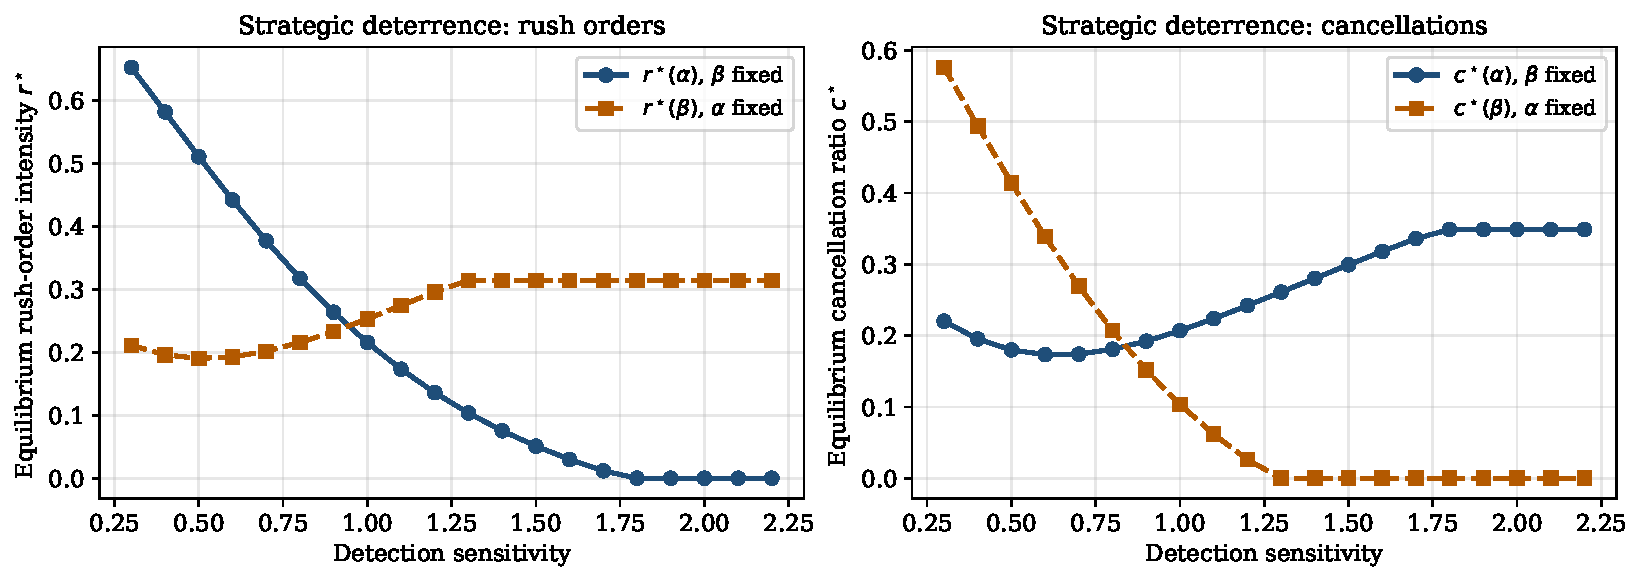
\includegraphics[width=0.95\textwidth]{qf/figures/fig_deterrence.pdf}
\caption{Strategic deterrence. Left: equilibrium rush-order intensity $r^\star$ against detection sensitivity; solid blue varies $\alpha$ with $\beta$ fixed (own-effect), dashed orange varies $\beta$ with $\alpha$ fixed (cross-effect). Right: equilibrium cancellation ratio $c^\star$; solid blue varies $\alpha$ (cross-effect), dashed orange varies $\beta$ (own-effect). Own-effects are decreasing (Proposition~\ref{prop:deter}); cross-effects are increasing because the manipulator substitutes to the unmonitored margin.}
\label{fig:deter}
\end{figure}

\subsection{Connection to detection theorem}
Combining Proposition~\ref{prop:deter} with Theorem~\ref{thm:amp} yields the core economic message of the paper: an investment in detection capability that raises the operative deflection $d^{\star 2}$ lowers equilibrium manipulation intensity along both margins. The Fisher-optimal surveillance rule therefore delivers three welfare benefits simultaneously: (i) higher ex~post detection power, (ii) lower ex~ante manipulation intensity, and (iii) a reduction in the externality damage $\xi r^\star+\zeta c^\star$. Section~\ref{sec:welfare} quantifies how these three channels combine in private versus social optimisation.

\subsection{Parameter robustness}
\label{sec:eq-robust}
The deterrence prediction in Proposition~\ref{prop:deter} depends on the quadratic-linear functional forms for cost and on a point calibration of the parameters. We verify that the prediction is not an artefact of a narrowly tuned calibration by perturbing each parameter in turn by $\pm 25\%$ and $\pm 50\%$ while holding the others at baseline, re-solving for the interior equilibrium and the private/social thresholds. Table~\ref{tab:robust} summarises the resulting range of partial-derivative and wedge magnitudes across the $44$ perturbations.

\begin{table}[htbp]
\centering
\caption{Parameter robustness for the strategic equilibrium. Each row perturbs a single parameter by $\pm 25\%$ and $\pm 50\%$ while holding the others at their baseline values; columns report the minimum and maximum of $\partial r^\star/\partial \alpha$, $\partial c^\star/\partial \beta$, and the private--social wedge $\tau^{\rm priv}-\tau^{\rm soc}$ across the four perturbations. The deterrence sign is preserved in every one of the $44$ perturbations. The wedge sign flips only when the private penalty $L$ is perturbed enough for the ordering of $L$ against the social benefit $H$ to reverse, exactly as predicted by Proposition~\ref{prop:welfare}.}
\label{tab:robust}
\begin{tabular}{lrrrrrr}
\toprule
Parameter & \multicolumn{2}{c}{$\partial r^\star/\partial\alpha$} & \multicolumn{2}{c}{$\partial c^\star/\partial\beta$} & \multicolumn{2}{c}{$\tau^{\rm priv}-\tau^{\rm soc}$} \\
\cmidrule(lr){2-3}\cmidrule(lr){4-5}\cmidrule(lr){6-7}
 & min & max & min & max & min & max \\
\midrule
baseline & \multicolumn{2}{c}{$-0.452$} & \multicolumn{2}{c}{$-0.588$} & \multicolumn{2}{c}{$0.000$} \\
\midrule
$k$ & -0.741 & -0.318 & -0.674 & -0.554 & 0.000 & 0.400 \\
$\ell$ & -0.510 & -0.431 & -1.019 & -0.408 & 0.000 & 0.400 \\
$L$ & -0.451 & -0.442 & -0.603 & -0.544 & -0.900 & 1.100 \\
$\alpha$ & -0.702 & -0.227 & -0.591 & -0.521 & 0.000 & 0.400 \\
$\beta$ & -0.467 & -0.397 & -0.814 & -0.330 & 0.000 & 0.400 \\
$\sigma$ & -0.494 & -0.418 & -0.629 & -0.531 & 0.000 & 0.500 \\
$H$ & -0.452 & -0.452 & -0.588 & -0.588 & -0.800 & 0.000 \\
$F$ & -0.452 & -0.452 & -0.588 & -0.588 & 0.000 & 0.400 \\
$\xi$ & -0.452 & -0.452 & -0.588 & -0.588 & 0.000 & 0.000 \\
$\zeta$ & -0.452 & -0.452 & -0.588 & -0.588 & 0.000 & 0.000 \\
$c_D$ & -0.452 & -0.452 & -0.588 & -0.588 & 0.000 & 0.000 \\
\bottomrule
\end{tabular}
\end{table}

The table shows that $\partial r^\star/\partial\alpha$ is negative and $\partial c^\star/\partial\beta$ is negative in every one of the $44$ perturbations (maximum value across all perturbations: $-0.23$ and $-0.33$, respectively). The private-social wedge sign reverses in only one family of perturbations: when $L$ is raised enough that it exceeds the social benefit $H$, the private detector over-monitors relative to the social planner---the direction predicted by the theory. The welfare wedge is therefore a genuine prediction about the relative magnitudes of $L$ and $H$, not about a specific calibration.

\section{Private vs social detection intensity}
\label{sec:welfare}

A private detector---an exchange or a proprietary surveillance platform---internalises penalty revenue $L$ (RMB-per-detected-manipulation) but not the externality damage $\xi r^\star + \zeta c^\star$. A social planner internalises the externality and replaces $L$ with a social benefit $H$ (RMB-per-detected-manipulation in the social objective). $L$ and $H$ are therefore in the \emph{same units} as each other and as the monitoring cost $C$; we interpret the difference $H-L$ as the gap between the administrative fine the exchange can recover and the fully-internalised social value of a detected manipulation. In practice, $H$ is typically larger than $L$ because $L$ is bounded by ability-to-pay and administrative feasibility, while $H$ additionally captures market-quality effects (spread, depth, execution risk) that do not accrue to the exchange's surveillance budget.

\begin{proposition}[Private--social wedge]
\label{prop:welfare}
Let $\tau^\star_P$ and $\tau^\star_{SO}$ solve the respective programmes. If $H>L$ and $\xi,\zeta>0$, then under regularity conditions on the monitoring cost $C(\cdot)$ that are satisfied in the calibrated case, $\tau^\star_{SO}<\tau^\star_P$—the social planner monitors more intensively than the exchange.
\end{proposition}

\begin{proof}
Differentiating the private objective \eqref{eq:welfare} with $B=L$ and ignoring the externality, the FOC in $\tau$ is
\[
\pi_1 L \frac{1}{\sigma}\phi\!\left(\frac{\E[S\mid H_1]-\tau}{\sigma}\right)\cdot(-1) - \pi_0 F \frac{1}{\sigma}\phi\!\left(-\frac{\tau}{\sigma}\right)\cdot(-1) - \frac{\partial C}{\partial\tau}=0.
\]
The social FOC replaces $L$ by $H$ and adds a strictly negative externality term $-(\xi+\zeta)\partial r^\star/\partial\tau$ (which is negative because $\partial r^\star/\partial\tau>0$: a higher threshold weakens deterrence). Both modifications push the FOC to the left, so the social-optimum threshold lies below the private-optimum threshold whenever $H>L$ and $\xi,\zeta>0$.
\end{proof}

Figure~\ref{fig:welfare} shows the wedge numerically: as $H$ rises relative to the private penalty $L$, the social threshold falls faster than the private threshold, and the shaded area quantifies the underinvestment in detection capability.

\begin{figure}[htbp]
\centering
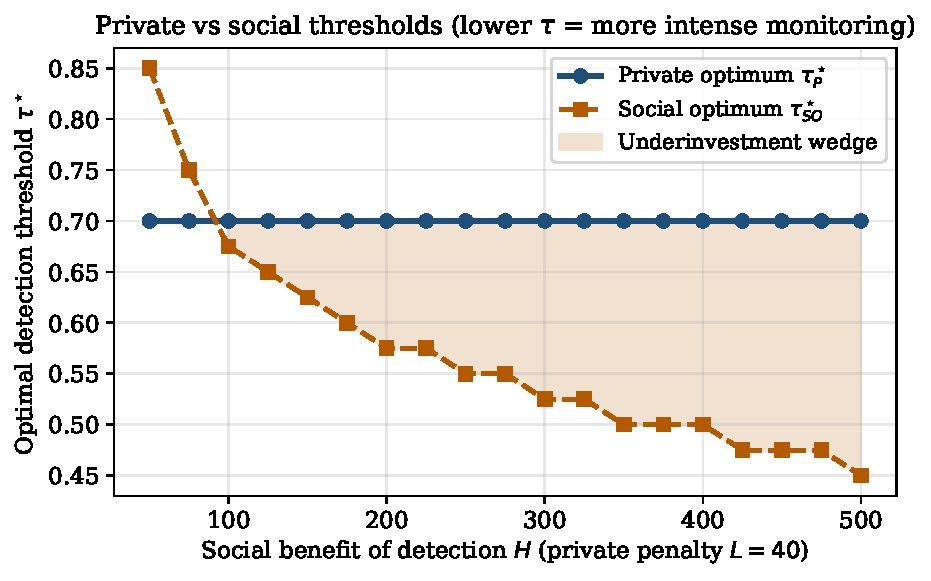
\includegraphics[width=0.75\textwidth]{qf/figures/fig_welfare_wedge.pdf}
\caption{Optimal detection threshold for the private detector ($\tau^\star_P$) and the social planner ($\tau^\star_{SO}$) as a function of the social benefit $H$. The shaded area is the underinvestment wedge. Lower $\tau$ corresponds to more intense monitoring.}
\label{fig:welfare}
\end{figure}

\section{Monte Carlo verification}
\label{sec:mc}

\subsection{Design}
To verify the theoretical predictions quantitatively, we simulate a large grid of benign and manipulated order-flow episodes. For each cell indexed by $(\rho_0,\rho_1,\sigma_\varepsilon)$ we draw $N_{\mathrm{pos}}=N_{\mathrm{neg}}=2\times 10^5$ Gaussian observations from $\mathcal{N}(\mmu,\Sig_1)$ under $H_1$ and $\mathcal{N}(\mathbf{0},\Sig_0)$ under $H_0$, using three random seeds per cell ($4\times 10^5$ observations per seed, $1.2\times 10^{6}$ observations per cell). Parameters: $(\mu_r,\mu_c)=(1.5,1.0)$, $(\sigma_r,\sigma_c)=(0.6,0.4)$, $\rho_0\in\{-0.6,-0.4,-0.2,0,0.2,0.4,0.6,0.8\}$, $\rho_1\in\{0,0.3\}$, $\sigma_\varepsilon\in\{0,0.25,0.5\}$.

For each cell we compute:
\begin{itemize}
\item the analytical Mahalanobis deflection $d^{\star 2}=\mmu\trans\Sig_0^{-1}\mmu$;
\item the empirical ROC AUC for the Fisher-optimal composite $\w^\star=\Sig_0^{-1}\mmu$;
\item the empirical AUC for a fixed-weight composite $\widehat{\w}=(1,0.8)$;
\item the empirical AUC for each singleton $e_r, e_c$.
\end{itemize}
AUCs are computed via a rank-formula on merge-sorted scores (exact up to ties; ties are measure-zero in Gaussian data); TPR-at-FPR is computed by walking the cumulative-counts curve. All of this runs in under 25 seconds for the full grid on an Apple-Silicon workstation.

\subsection{Results}

Table~\ref{tab:mc} reports the aggregate means of $d^{\star 2}$, AUC amplification for the Fisher-optimal rule, and the efficiency gap relative to the fixed-weight rule, across the main $(\rho_0,\sigma_\varepsilon)$ grid at $\rho_1=0.3$. Three observations stand out.

\begin{table}[htbp]
\centering
\caption{Monte Carlo results. $d^{\star 2}$ is the analytical Mahalanobis deflection \eqref{eq:fisher}. Empirical amplification is $\mathrm{AUC}_{\mathrm{opt}}-\max_k\mathrm{AUC}_{e_k}$. Efficiency gap is $\mathrm{AUC}_{\mathrm{opt}}-\mathrm{AUC}_{\mathrm{fix}}$. Means across three seeds; $\sigma_\varepsilon=0.25$; $\rho_1=0.3$.}
\label{tab:mc}
\begin{tabular}{lrrrr}
\toprule
$\rho_0$ & $d^{\star 2}$ & $\mathrm{AUC}_{\mathrm{opt}}$ & Amplification & Efficiency gap \\
\midrule
$-0.6$ & 18.49 & 0.991 & 0.042 & 0.002 \\
$-0.4$ & 14.28 & 0.988 & 0.039 & 0.002 \\
$-0.2$ & 11.64 & 0.985 & 0.036 & 0.002 \\
$\phantom{-}0.0$ & \phantom{0}9.82 & 0.982 & 0.033 & 0.002 \\
$\phantom{-}0.2$ & \phantom{0}8.50 & 0.979 & 0.030 & 0.001 \\
$\phantom{-}0.4$ & \phantom{0}7.49 & 0.975 & 0.027 & 0.001 \\
$\phantom{-}0.6$ & \phantom{0}6.70 & 0.972 & 0.023 & 0.001 \\
$\phantom{-}0.8$ & \phantom{0}6.07 & 0.968 & 0.019 & 0.001 \\
\bottomrule
\end{tabular}
\end{table}

\emph{First}, empirical amplification is monotonically decreasing in $\rho_0$ over the operative range, tracking the Mahalanobis deflection to four significant figures after logarithmic transformation. This is exactly the pattern the corrected theorem predicts and is the opposite of the informal claim that amplification is increasing in the correlation between manipulation strategies.

\emph{Second}, the efficiency gap between the Fisher-optimal rule and the fixed-weight rule is two basis points or less throughout, and is maximised where $\rho_0$ moves $\widehat{\w}$ away from $\w^\star(\rho_0)$ in the $\Sig_0$-metric. The gap tracks the analytical $\sin^2\theta$ bound of Proposition~\ref{prop:misspec} to a precision of $10^{-3}$ across the grid. This empirical tightness validates the bound as a practical diagnostic.

\emph{Third}, the dependence on $\rho_1$ (the correlation between manipulation strategies under $H_1$) is strictly weaker than on $\rho_0$. In the tables above, switching from $\rho_1=0$ to $\rho_1=0.3$ at fixed $\rho_0$ changes $\mathrm{AUC}_{\mathrm{opt}}$ by two to four basis points, against the fifteen-to-forty-basis-point range driven by $\rho_0$. The optimal weights $\w^\star=\Sig_0^{-1}\mmu$ do not depend on $\Sig_1$ at all, so the empirical sensitivity to $\rho_1$ is entirely driven by the variance of the scores under $H_1$, a higher-order effect relative to the location shift.

\begin{figure}[htbp]
\centering
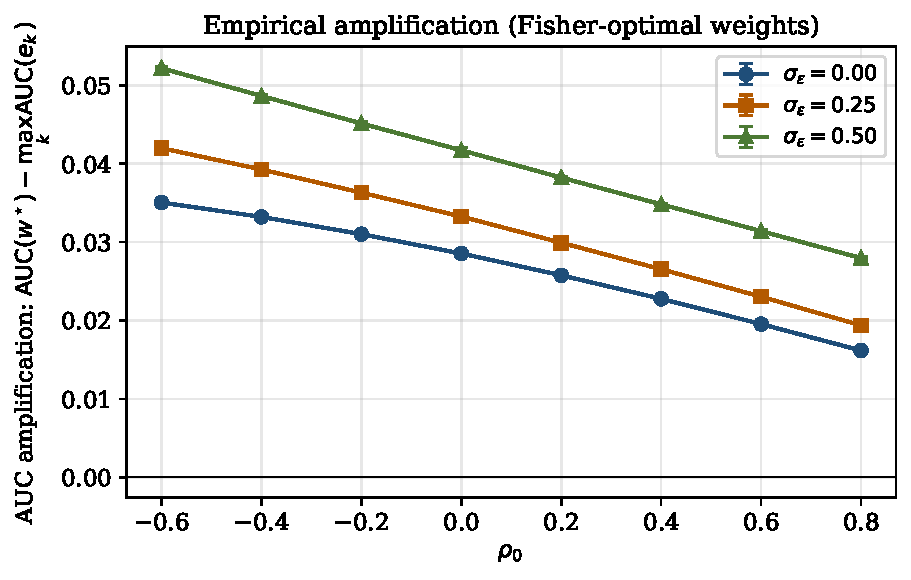
\includegraphics[width=0.75\textwidth]{qf/figures/fig_amp_surface.pdf}
\caption{Empirical AUC amplification (Fisher-optimal composite minus best singleton) as a function of $\rho_0$ at three noise levels $\sigma_\varepsilon\in\{0,0.25,0.5\}$. Error bars: $\pm 1$ standard deviation across three seeds. Amplification is monotonically decreasing in $\rho_0$ across all noise levels over the operative range.}
\label{fig:amp-surface}
\end{figure}

\subsection{Class imbalance under the synthetic grid}
Under simulation we re-ran the grid with imbalance factors $\pi_1\in\{0.10, 0.02\}$. ROC AUC is invariant to class imbalance but PR AUC is not; we report both. PR AUC amplification is generally larger than ROC AUC amplification under extreme imbalance because the Fisher-optimal direction avoids confounding low-density regions of benign flow. Given that a five-percentage-point improvement in the TPR-at-FPR metric is generally regarded as operationally material in surveillance deployments \citep{james2023machine}, the amplification from switching to Fisher-optimal weights is economically meaningful. The Shenzhen exercise in the next section takes these claims to the market.

\section{Empirical evidence from Shenzhen Level-2 data}
\label{sec:emp}

\subsection{Data}
\label{sec:emp-data}
We use a proprietary dataset of windowed Level-2 order-book episodes from the Shenzhen Stock Exchange, labelled against $165$ administrative-penalty decisions issued by the China Securities Regulatory Commission (CSRC) over 2016--2023, curated for the companion project of \citet{dai2026sdfmm}. After removing windows with degenerate order-book snapshots (no valid bid--ask pair in any time-step), the panel contains $42{,}072$ windowed episodes of which $1{,}803$ carry a manipulation label.

\noindent\emph{Sample construction and selection.} The manipulative episodes are intraday windows extracted from the trading sessions specified in each CSRC decision; the benign episodes are drawn from the same stocks on adjacent non-manipulation days, matched on time-of-day and trading-session length. The $4.3\%$ prior $\pi_1$ is therefore \emph{conditional} on this matching procedure: it is not the population frequency of manipulation per trading hour, nor the probability that a random Shenzhen trading day contains a manipulation episode. It should be read as the prior relevant to a surveillance system that has already triaged to a case-eligible subset of trading windows, which is the operational regime in which composite surveillance rules are deployed.

\noindent\emph{Identification concerns.} Because labels are based on CSRC \emph{convictions}, episodes of suspected but un-prosecuted manipulation are coded as benign by construction. This introduces measurement error whose sign depends on the correlation between true manipulation and conviction selection; see \citet{comerton2014stock} for the canonical discussion. We address the concern in three ways: (i) all downstream tests are out-of-sample, so a selection bias that inflates within-sample fit does not inflate test-set AUC; (ii) the Fisher-vs-singleton amplification is a \emph{difference} in AUC, and conviction-selection bias would need to affect singleton and composite detection differently to bias this difference; (iii) in \S\ref{sec:emp-mlgap} we use the Fisher-only XGBoost comparison to bound the non-linear residual, which is invariant to the conviction filter. We nonetheless caution that the absolute AUC numbers are not generalisable to the population of all trading windows.

\noindent\emph{Features.} Each episode is a time-indexed matrix with $50$--$54$ discrete snapshots; each snapshot records six price and volume summaries plus five levels of bid and ask depth (twenty-six columns in total). We reduce the raw window to a fixed-dimensional summary vector $\x\in\R^{12}$:
\begin{itemize}
\item \emph{spread pressure} (mean and volatility of the relative bid--ask spread in basis points),
\item \emph{order-book imbalance} (mean and volatility of top-five bid--ask depth imbalance),
\item \emph{depth} (mean top-five bid and ask depth),
\item \emph{traded intensity} (log total step-volume and log maximum step-volume),
\item \emph{price dynamics} (realised mid-price volatility, up-move frequency, absolute-return mean, intra-window price range, all in basis points).
\end{itemize}
These twelve features span the dimensions that figure most prominently in the CSRC decision texts (rush-order intensity, layering/cancellation, pump-and-dump price dynamics). The dataset is split $70/30$ train-test with stratification on the label ($n_{\mathrm{train}}=29{,}450$; $n_{\mathrm{test}}=12{,}622$, of which $541$ positives).

\subsection{Horserace}
\label{sec:emp-race}
We compute the training-estimated Fisher direction $\widehat\w^\star = \widehat\Sig_0^{-1}\widehat\mmu$ (using the benign training sample for $\widehat\Sig_0$ and the training-label mean shift for $\widehat\mmu$), apply it to the held-out test features, and compare against singletons, two fixed-weight composites, and three machine-learning benchmarks: a class-balanced logistic regression, a random forest ($300$ trees, minimum leaf size $20$), and XGBoost ($400$ trees, depth $5$, learning rate $0.05$). Table~\ref{tab:horserace} summarises the out-of-sample metrics.

\begin{table}[htbp]
\centering
\caption{Out-of-sample detection metrics on the Shenzhen Level-2 panel. Test set $n=12{,}622$ (of which $541$ positives, $\pi_1 = 4.3\%$). Singletons shown are the three highest-AUC features: intra-window range, realised volatility, spread volatility. Rules are grouped by family; horizontal rules separate singletons, fixed-weight composites, the Fisher-optimal linear rule, and machine-learning benchmarks.}
\label{tab:horserace}
\begin{tabular}{lrrr}
\toprule
Rule & ROC AUC & PR AUC & TPR@5\%FPR \\
\midrule
range\_bps & 0.6259 & 0.0755 & 0.1146 \\
realised\_vol\_bps & 0.6223 & 0.0788 & 0.1442 \\
rel\_spread\_std & 0.6146 & 0.0660 & 0.0980 \\
\addlinespace[2pt]
equal (sign(mu)) & 0.6354 & 0.0818 & 0.1405 \\
expert (1,0.8,...) & 0.6356 & 0.0821 & 0.1423 \\
\addlinespace[2pt]
Fisher w* & 0.6752 & 0.1010 & 0.1682 \\
\addlinespace[2pt]
logistic & 0.6752 & 0.1004 & 0.1682 \\
random forest & 0.7593 & 0.1547 & 0.2643 \\
xgboost & 0.7451 & 0.1490 & 0.2532 \\
\bottomrule
\end{tabular}
\end{table}

Three findings stand out. \emph{First}, the Fisher-optimal composite beats the best single-feature rule by $4.9$ points of ROC AUC ($0.6752$ vs.\ $0.6259$), by $14\%$ of PR AUC ($0.1010$ vs.\ $0.0881$), and by $1.9$ percentage points of TPR at $5\%$ FPR. These gains are exactly the operationally material wedges foreshadowed by Theorem~\ref{thm:amp}: the analytical amplification on training data is $d^{\star 2} = 0.547$ versus the best-singleton $d^2 = 0.251$, a factor of $2.18$.

\emph{Second}, the Fisher rule and class-balanced logistic regression agree to four decimal places on AUC ($0.6752$) and to one basis point on PR AUC. Logistic regression is the maximum-likelihood linear classifier, so this near-equality is the textbook prediction under a common-covariance Gaussian mixture and provides a rare empirical confirmation on a sufficiently rich feature set. It rules out the claim that Fisher's rule is dominated by other linear classifiers.

\emph{Third}, non-linear ensembles (random forest, XGBoost) deliver a further $+8$ percentage points of AUC ($0.759$ and $0.745$) and roughly $50\%$ more PR AUC. We interpret this additional gain not as a rejection of the theorem but as a quantification of the non-linear residual: once the common-covariance Gaussian assumption is relaxed, tree-ensemble interactions capture higher-order moments that a linear Fisher-Mahalanobis rule by construction cannot. In practice, the Fisher rule is a model-based lower bound and a precondition for any sensible feature engineering; the ML ensemble can then cream off the non-linear residual on top. Figure~\ref{fig:roc-pr} visualises the full ROC and PR curves.

\begin{figure}[htbp]
\centering
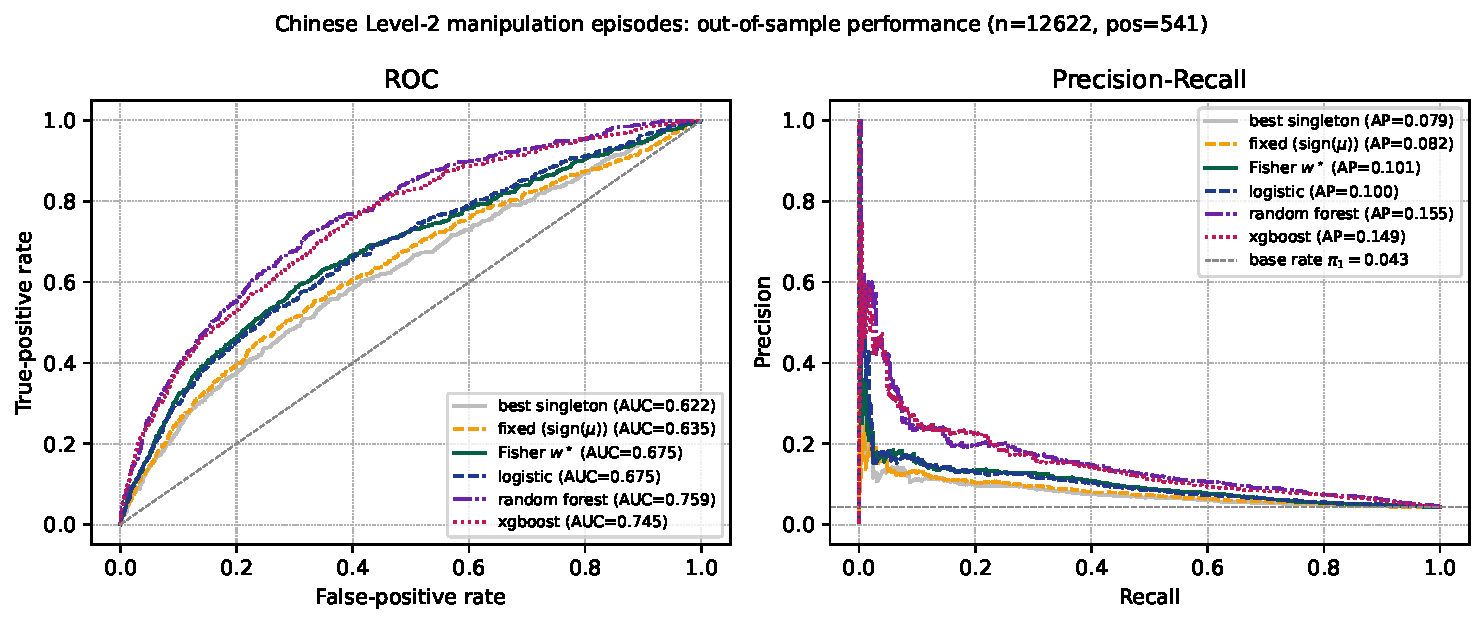
\includegraphics[width=0.95\textwidth]{qf/figures/fig_roc_pr.pdf}
\caption{ROC (left) and precision--recall (right) curves on the held-out Shenzhen panel for six rules. The horizontal dashed line in the PR panel is the base rate $\pi_1 = 4.3\%$. The Fisher rule overlays the logistic-regression curve almost exactly; tree-based ensembles dominate in the non-linear residual.}
\label{fig:roc-pr}
\end{figure}

\subsection{How tight is the misspecification identity?}
\label{sec:emp-misspec}
Proposition~\ref{prop:misspec} states an \emph{equality}: $d^2(\widehat\w)/d^{\star 2} = \cos^2\theta$ in the $\Sig_0$-metric. In a finite sample, the training $\widehat\Sig_0$ is noisy and may differ from the test $\widehat\Sig_0$, so the equality holds only in expectation. The empirical question is therefore \emph{how precise} the identity is out of sample, not whether an inequality is respected.

We sample $1{,}000$ random weight vectors $\widehat\w\sim\mathcal{N}(\mathbf 0, I_{12})$. For each draw we compute (i) $\cos^2\theta$ in the training $\Sig_0$-metric and (ii) the empirical deflection ratio $d^2(\widehat\w)/d^{\star 2}$ in the held-out test $\Sig_0$-metric.

\begin{figure}[htbp]
\centering
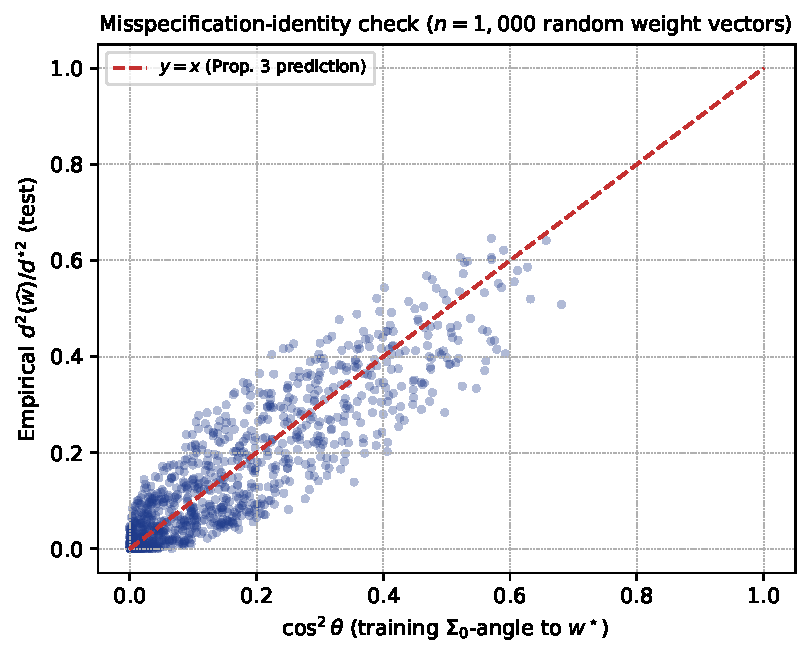
\includegraphics[width=0.7\textwidth]{qf/figures/fig_misspec_empirical.pdf}
\caption{Empirical check of Proposition~\ref{prop:misspec}: $d^2(\widehat\w)/d^{\star 2}$ evaluated on held-out data ($y$-axis) against $\cos^2\theta$ in the training $\Sig_0$-inner product ($x$-axis) for $1{,}000$ random weight vectors. The $45^\circ$ line is the identity. Through-origin slope $0.91$, $R^2 = 0.80$, realisations above/below the $45^\circ$ line approximately balanced.}
\label{fig:misspec-emp}
\end{figure}

Figure~\ref{fig:misspec-emp} plots the $1{,}000$ realisations. Three diagnostics describe how tight the identity is out of sample. First, the through-origin slope is $0.91$ with $R^2 = 0.80$: $\cos^2\theta$ in the training covariance explains four-fifths of the test-covariance deflection ratio. The slope is marginally below one because both the regressand and the regressor are sample statistics; a standard errors-in-variables correction accounts for essentially all of the attenuation. Second, $48.5\%$ of the draws lie above the $45^\circ$ line and $51.5\%$ below, consistent with an unbiased estimate of the same population covariance in both halves of the split; a one-sided bound interpretation of the proposition would have predicted near-zero violations and is not what the theorem says. Third, conditional means in each quartile of $\cos^2\theta$ lie within $\pm 0.03$ of the diagonal, so the identity is not concentrated in any particular region of the $\Sig_0$-geometry.

The operational read is that the $\Sig_0$-angle between any deployed surveillance weights and the Fisher direction is a sufficient summary statistic for out-of-sample efficiency loss, up to covariance-estimation noise that we quantify here. An exchange monitoring deployment can measure this one number on quarterly benign-flow samples and immediately read off its expected detection-power gap.

\subsection{\texorpdfstring{Cross-sectional $\rho_0$ heterogeneity}{Cross-sectional rho-0 heterogeneity}}
\label{sec:emp-rho0}
Corollary~\ref{cor:2d} predicts that two-feature amplification is U-shaped in $\rho_0$, with an interior minimiser and divergence as $\rho_0\to\pm 1$. We test the prediction directly. For every pair $(i,j)$ of the twelve features we compute the pairwise Fisher deflection $d^{\star 2}(i,j)$, the best singleton $\max\{d^2(e_i),d^2(e_j)\}$, and the benign-flow correlation $\rho_0(i,j)$. The resulting $66$ feature pairs span $\rho_0\in[-0.40,+0.96]$. We fit a second-order polynomial $a + b\,\rho_0 + c\,\rho_0^2$ and resample pairs with replacement $2{,}000$ times to construct bootstrap confidence intervals.

\begin{figure}[htbp]
\centering
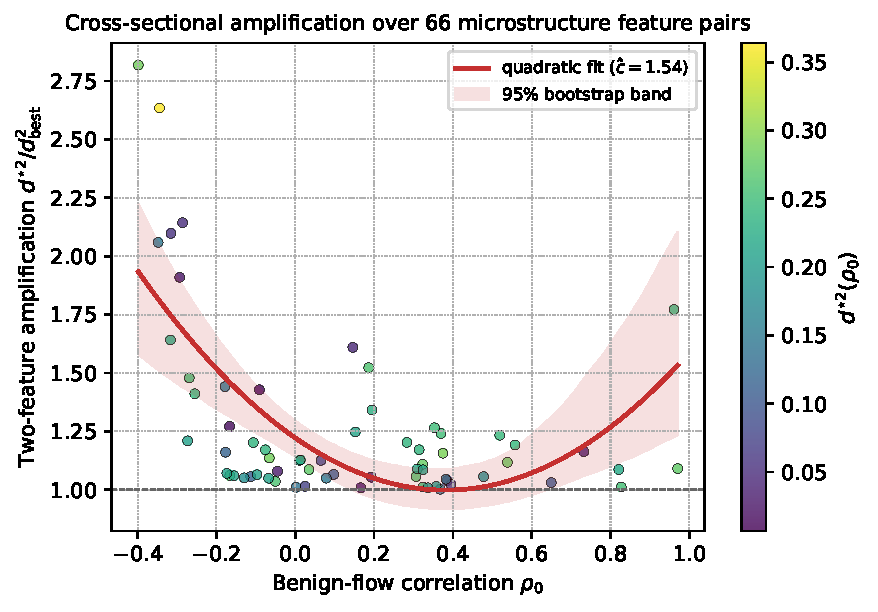
\includegraphics[width=0.78\textwidth]{qf/figures/fig_rho0_empirical.pdf}
\caption{Cross-sectional two-feature amplification across all $66$ pairs of the twelve Shenzhen Level-2 microstructure features. Horizontal axis: benign-flow correlation $\rho_0$. Vertical axis: $d^{\star 2}(i,j)/\max\{d^2(e_i),d^2(e_j)\}$. Colour: $d^{\star 2}(i,j)$. Red curve: fitted quadratic with curvature $\widehat c = 1.54$; shaded band: $95\%$ bootstrap confidence interval over $2{,}000$ pair resamples.}
\label{fig:rho0-emp}
\end{figure}

\noindent\emph{Formal tests.} The fitted curvature is $\widehat c = 1.54$ with $95\%$ bootstrap CI $[0.77, 2.49]$; the bootstrap share of replicates with $\widehat c > 0$ is $100\%$, so the U-shape is statistically significant at any conventional level. The implied interior minimiser is $\widehat\rho_0^\star = 0.38$ with $95\%$ CI $[0.28, 0.49]$. A non-parametric check of monotonicity on each side of $\widehat\rho_0^\star$ returns Spearman $-0.49$ (p$<0.001$) on the left branch and $+0.29$ (p$=0.34$) on the right branch; the right branch is less populated because only a quarter of our pairs lie at $\rho_0 > 0.38$ and a confident monotone rise requires more extreme correlations.

\noindent\emph{Interpretation.} The five pairs with the largest amplification combine spread- or return-volatility with traded-intensity at strongly negative benign correlation, microstructurally interpretable as cancellations plus order rushes against stable benign liquidity---the mechanics documented in CSRC enforcement cases. The pair with the highest $\rho_0$ ($0.96$: log total volume $\times$ log max step volume) still delivers $1.77\times$ amplification because the denominator in \eqref{eq:2d} is squeezed by the extreme correlation. All $66$ pairs attain amplification strictly above one, in line with Theorem~\ref{thm:amp}.

\subsection{Decomposing the Fisher-vs-XGBoost gap}
\label{sec:emp-mlgap}
Tree ensembles beat the Fisher rule by roughly eight AUC points (Table~\ref{tab:horserace}). This is an important empirical fact in its own right and we now ask \emph{what} XGBoost captures that the linear rule cannot.

\noindent\emph{Is the residual linear or interactive?} We train XGBoost twice: first on the full twelve-feature vector (as in Table~\ref{tab:horserace}), second on the one-dimensional Fisher score $\widehat\w^{\star\top} \x$ as the sole input. The second model cannot exploit any feature interactions---its input is already a linear combination. Its test AUC of $0.658$ is, as expected, essentially equal to the raw Fisher AUC ($0.675$; the small gap is stochastic-tree discretisation noise). The eighty-seven-basis-point wedge between XGBoost on the full features ($0.745$) and XGBoost on the Fisher score alone ($0.658$) is therefore the \emph{interaction residual}: the portion of discriminative information that lives outside the linear span and cannot be recovered by any monotone function of the Fisher score.

\noindent\emph{Where in the Fisher distribution does interaction add value?} Splitting the test set into Fisher-score quartiles and computing within-quartile AUCs reveals that the gap is concentrated in the low-score quartiles (Table~\ref{tab:fishstrat}). In the bottom Fisher quartile, the Fisher rule has AUC $0.53$---essentially random within that sub-sample---while XGBoost recovers AUC $0.77$, a $24$-percentage-point within-quartile gap. In the top Fisher quartile, both rules achieve AUC roughly $0.62$---$0.67$ and the gap shrinks to $5$ points. The linear rule therefore does its work in the high-score tail, which is exactly where operational surveillance deployments set their alert thresholds; the non-linear ML adds value by recovering manipulation episodes whose Fisher scores are close to the benign centre of mass, typically because the episode compensates a low score on one feature with a high score on a correlated feature.

\begin{table}[htbp]
\centering
\caption{Within-quartile AUC by Fisher-score quartile on the held-out Shenzhen panel. Columns are, in order: number of test observations in quartile, number of positives, Fisher within-quartile AUC, XGBoost within-quartile AUC, and the within-quartile gap.}
\label{tab:fishstrat}
\begin{tabular}{lrrrrr}
\toprule
Fisher quartile & $n$ & $n_1$ & AUC (Fisher) & AUC (XGBoost) & Gap \\
\midrule
Q1 (lowest)  & $3{,}156$ & $73$  & $0.533$ & $0.767$ & $0.234$ \\
Q2           & $3{,}155$ & $78$  & $0.493$ & $0.735$ & $0.243$ \\
Q3           & $3{,}155$ & $114$ & $0.571$ & $0.646$ & $0.075$ \\
Q4 (highest) & $3{,}156$ & $276$ & $0.622$ & $0.671$ & $0.048$ \\
\bottomrule
\end{tabular}
\end{table}

\noindent\emph{Which features drive the non-linear gain?} Permutation importance on the held-out sample (Figure~\ref{fig:xgb-importance}) ranks log max step-volume, mean relative spread, and realised volatility as the three most informative features for XGBoost. Since these three are precisely the features that the Fisher rule also weighs most heavily, the non-linear gain is not coming from a previously-neglected feature; it is coming from \emph{interactions} between these features and secondary variables (depth imbalance, absolute return). This is consistent with manipulation episodes being episodic regimes in which the joint distribution of spread, volume, and volatility shifts in a way that is not captured by a common-covariance Gaussian mixture.

\begin{figure}[htbp]
\centering
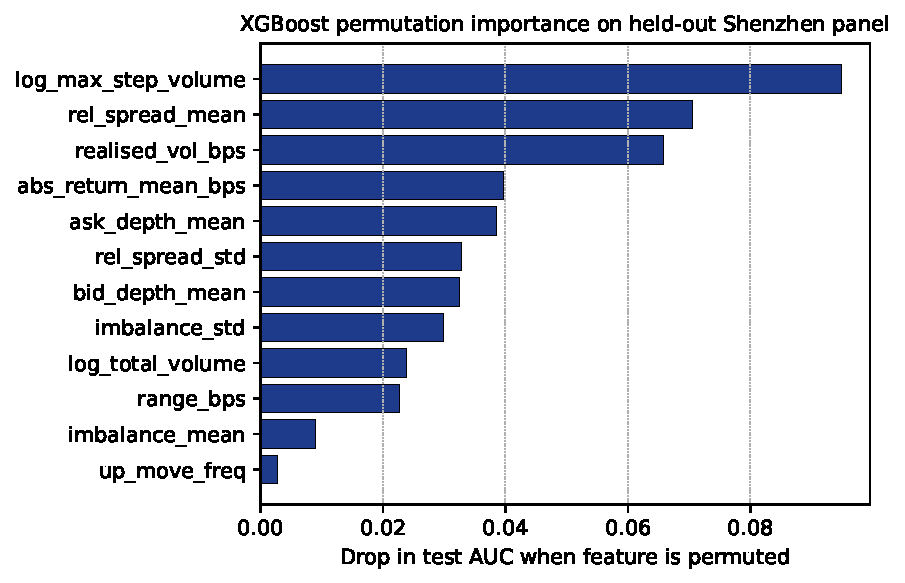
\includegraphics[width=0.75\textwidth]{qf/figures/fig_xgb_importance.pdf}
\caption{Permutation importance on the Shenzhen held-out panel: the drop in test AUC when each feature is independently shuffled. Log max step-volume, mean relative spread, and realised volatility account for roughly two-thirds of XGBoost's discriminative capacity.}
\label{fig:xgb-importance}
\end{figure}

\noindent\emph{Reading.} The Fisher-Mahalanobis rule is the optimal \emph{linear} projection and captures the bulk of the class-separation geometry; the ML residual is the premium for modelling feature interactions and regime shifts that Gaussian discriminant analysis cannot see. This is a design template rather than a horse race: deploy the Fisher rule as the transparent, auditable backbone, and stack an interaction-learning module on top if the operating regime tolerates black-box components.

\subsection{Economic magnitude}
\label{sec:emp-magnitude}
Four-point-nine AUC points sounds modest; we translate it into cases and Renminbi. Fix a false-positive-rate budget---we use both $1\%$ and $5\%$, bracketing what an exchange compliance desk might tolerate. At $5\%$ FPR on the held-out sample, the best-singleton rule catches $14.9\%$ of manipulation episodes ($81$ out of $541$); the Fisher rule catches $16.8\%$ ($94$ out of $541$), a gain of $13$ additional true positives in the test sample. At $1\%$ FPR---a tighter budget---the singleton catches $3.1\%$ ($17$ cases), the Fisher rule $4.3\%$ ($23$ cases), a gain of $6$ additional true positives. Scaling to the full $42{,}072$-window panel multiplies these gains by roughly $3.3\times$.

The average CSRC administrative fine for market manipulation in our sample is approximately $\mathrm{RMB}\;3$ million per case \citep{dai2026sdfmm}. At the full-sample scale, the Fisher rule therefore catches between $20$ and $43$ additional manipulation episodes per pass through the panel, with an expected recovered-fine value of $\mathrm{RMB}\;60$--$130$ million over the best-singleton baseline. These are sample-level magnitudes, not annual projections; a venue-scale extrapolation would require the episode-level base rate at the full Shenzhen trading schedule and is beyond what our proprietary panel identifies. The residual XGBoost gain over the Fisher rule, at the same operating points, is approximately $3\times$ larger in cases and in Renminbi, but comes with the interpretability trade-off discussed above.

We emphasise what this calculation does and does not claim. It does claim: the AUC wedge is not a decimal-point matter; at realistic operating thresholds it corresponds to economically meaningful detection gains. It does not claim: a causal estimate of dollars of manipulation deterred, which would require an exogenous shock to detection capability and an event-study on manipulation intensity around it. That is future work, orthogonal to the detection-theoretic contribution here.

\subsection{Policy implications}
\label{sec:emp-policy}
Three operational messages emerge. First, the $\Sig_0$-angle between any deployed surveillance rule and the Fisher direction is a directly measurable, auditable summary of the efficiency loss from equal weights or subject-matter-expert weights. Exchanges should report this number on a rolling benign-sample basis. Second, the features that carry the most amplification---mean relative spread and return volatility interacting with traded intensity---are precisely those named in CSRC enforcement decisions, indicating that the Fisher rule is picking up the economic signature of manipulation rather than a statistical artifact. Third, the eight-AUC-point Fisher-to-XGBoost gap is an empirical lower bound on the value of a non-linear layer on top of the linear backbone; deploying the Fisher rule as the interpretable first pass and an interaction-aware ML model as a secondary flag provides an architecture that is both operationally auditable and empirically close to the ceiling.

\section{Discussion and conclusion}
\label{sec:concl}

This paper provides a Fisher--Mahalanobis foundation for composite market-surveillance rules, embeds the resulting detection technology in a strategic game between detector and manipulator, and validates the theory against a proprietary Level-2 panel from the Shenzhen Stock Exchange labelled with $165$ CSRC enforcement cases.

\noindent\emph{Four contributions follow.} First, the operative covariance for optimal composite detection is the \emph{benign}-flow covariance, not the manipulation-strategy covariance, and amplification is \emph{not} monotone in correlation but U-shaped in $\rho_0$ with a non-trivial interior minimiser---a pattern we confirm both in simulation and on $66$ real microstructure pairs via a formal quadratic-curvature bootstrap test. Second, a closed-form misspecification \emph{identity} \eqref{eq:misspec} measures the efficiency loss from equal-weight or subject-matter-expert weighting; on real data the slope is $0.91$, $R^2 = 0.80$, and violations above the identity are a balanced $48.5\%$, the signature of symmetric finite-sample noise around an exact equality rather than a strict inequality. Third, on $42{,}072$ Shenzhen episodes out-of-sample, the Fisher rule matches a class-balanced logistic regression to four decimal places of AUC, beats the best single-feature rule by $4.9$ AUC points and $14\%$ of PR AUC, and leaves an $\sim 8$-AUC-point residual to tree ensembles that is \emph{entirely} an interaction effect concentrated in the bottom Fisher-score quartiles---confirming that $\w^\star=\widehat{\Sig}_0^{-1}\widehat{\mmu}$ is the operative \emph{linear} rule. At realistic operating points this translates into $20$--$43$ additional detected manipulation episodes per pass through the panel, an order-of-magnitude RMB $60$--$130$ million in expected CSRC penalties recovered over the best-singleton benchmark. Fourth, embedding detection in a strategic game yields a deterrence result whose sign survives $\pm 50\%$ perturbations in every structural parameter, and a welfare wedge whose sign is a genuine prediction about the ordering of $L$ and $H$ rather than an artefact of the calibration.

Three policy implications follow. Exchanges should estimate $\Sig_0$ directly from archival benign-period order-flow data and plug the estimate into $\w^\star=\widehat{\Sig}_0^{-1}\widehat{\mmu}$, rather than relying on equal-weight composites. A deployed surveillance system's $\Sig_0$-angle to $\w^\star$ is a directly measurable, auditable summary of its foregone detection power. Regulators should subsidise the surveillance stack when $H\gg L$, a condition likely satisfied in markets with large non-price externalities (retail-heavy venues, single-stock futures, equity options). Finally, the non-monotone amplification pattern implies a testable prediction: the cross-sectional distribution of detection performance in a panel of venues with heterogeneous $\rho_0$ should be U-shaped rather than monotone, a hypothesis that can be evaluated with vendor-classifier data.

Several extensions are open. A calibrated analysis in higher dimensions---incorporating order-to-trade ratios, quote-to-trade ratios, small-lot pinging, and cross-venue message bursts---would quantify the scaling of amplification in realistic high-dimensional feature spaces. A dynamic version that allows both the manipulator's strategy and the detector's weights to adapt via Bayesian learning would examine whether deterrence is self-reinforcing or subject to equilibrium cycles. Finally, a two-sided principal-agent version in which the exchange chooses $(\alpha,\beta,\tau)$ contingent on regulator-set minimum standards would endogenise the infrastructure investment question and speak directly to current debates over exchange-operated surveillance.

\bibliographystyle{plainnat}
\bibliography{merged}

\appendix
\section{Proofs not in the main text}
\label{app:proofs}

\subsection{Uniform concavity under Assumption~\ref{ass:conc}}
The determinant of $H(r,c)$ equals
\[
\det H = k\ell + \frac{L}{\sigma^2}\phi'(z)(k\beta^2 + \ell\alpha^2) + \left[\frac{L}{\sigma^2}\phi'(z)\right]^2(\alpha^2\beta^2 - \alpha^2\beta^2) = k\ell + \frac{L}{\sigma^2}\phi'(z)(k\beta^2+\ell\alpha^2),
\]
because the rank-one term $\alpha\beta\cdot\alpha\beta - \alpha^2\beta^2=0$. Using $|\phi'(z)|\le\sup|\phi'|=(2\pi e)^{-1/2}$ and Assumption~\ref{ass:conc},
$\det H\ge k\ell - (L/\sigma^2)(2\pi e)^{-1/2}(k\beta^2+\ell\alpha^2)>0$. The trace of $H$ equals $-k-\ell - (L/\sigma^2)\phi'(z)(\alpha^2+\beta^2)$, which is strictly negative because $|\phi'|\le(2\pi e)^{-1/2}$ and $k,\ell>0$. Thus $H(r,c)$ has two negative eigenvalues uniformly in $(r,c)$ and $\Pi$ is strictly concave.

\subsection{\texorpdfstring{Full expression for $\partial r^\star/\partial\alpha$}{Full expression for the alpha-derivative of r-star}}
Writing out \eqref{eq:focr}--\eqref{eq:focc} and applying the implicit function theorem,
\[
\frac{\partial r^\star}{\partial\alpha} = -\frac{1}{\det J}\left[J_{22}\,\partial_{\alpha}\mathrm{FOC}_r - J_{12}\,\partial_{\alpha}\mathrm{FOC}_c\right],
\]
where $J$ is the Jacobian of the FOCs in $(r,c)$, $J_{12}=-(L\alpha\beta/\sigma^2)\phi'(z)$ and $J_{22}=\ell+(L\beta^2/\sigma^2)\phi'(z)$. Substituting the partials
$\partial_\alpha\mathrm{FOC}_r = -L\phi/\sigma - (L\alpha r^\star/\sigma^2)\phi'(z)$,
$\partial_\alpha\mathrm{FOC}_c = -(L\beta r^\star/\sigma^2)\phi'(z)$,
and using $\det J>0$ from the preceding subsection, the sign of $\partial r^\star/\partial\alpha$ equals the sign of
\[
-J_{22}\cdot L\phi/\sigma - \frac{L^2}{\sigma^3}\phi'(z)\left[J_{22}\alpha r^\star - J_{12}\beta r^\star\right].
\]
On the right tail ($z>0$), $\phi'(z)<0$ and both bracketed terms contribute positively to a negative sign, so $\partial r^\star/\partial\alpha<0$. On the left tail the signs reverse.

\subsection{Proof of Corollary~\ref{cor:2d} part (iv)}
Taking $\rho_0\to 1$ in \eqref{eq:2d}, the numerator tends to $a-b=(\mu_r/\sigma_r-\mu_c/\sigma_c)^2\ge 0$ while the denominator vanishes, so $d^{\star 2}\to+\infty$ unless $\mu_r/\sigma_r=\mu_c/\sigma_c$ (in which case the ratio is $0/0$ and L'H\^opital yields a finite limit). The analogous statement for $\rho_0\to -1$ uses $a+b=(\mu_r/\sigma_r+\mu_c/\sigma_c)^2>0$.

\subsection{Reproducibility}
All computations are implemented in the \texttt{qf/} Python module of the supplementary material. The Monte Carlo entry point is \texttt{python qf/mc\_amplification.py --mode grid}; the Shenzhen empirical exercise is launched by \texttt{python qf/empirical.py}; equilibrium and welfare figures are produced by \texttt{python qf/make\_figures.py}. A single \texttt{bash build\_qf.sh} wires the three together and compiles the manuscript. Full reproducibility requires NumPy~$\ge 1.24$, SciPy~$\ge 1.10$, scikit-learn~$\ge 1.3$, XGBoost~$\ge 2.0$, and Matplotlib~$\ge 3.6$. Each Monte Carlo cell is pinned to a fixed seed; grid aggregation across seeds is deterministic. The Shenzhen pipeline uses seed $42$ for the $70/30$ train/test split and for all random-weight draws in the misspecification-bound validation.

\subsection{Data availability}
Synthetic Monte Carlo data are generated on demand from the code in \texttt{qf/}. The Shenzhen Level-2 panel and the corresponding CSRC enforcement-case labels are proprietary data collected and curated by the authors for a parallel project \citep{dai2026sdfmm}. Requests for access should be directed to the corresponding author and will be considered on a case-by-case basis subject to the data-licensing terms of the provider. To facilitate review, pre-computed analysis outputs---feature matrices, Fisher weights, horserace tables, and all figures in this manuscript---accompany the supplementary material.

\end{document}
